\documentclass[10pt,aspectratio=169,usenames,dvipsnames]{beamer} % handout

% https://de.overleaf.com/latex/templates/metropolis-beamer-theme/qzyvdhrntfmr
\usetheme[progressbar=frametitle]{metropolis}
\usepackage{appendixnumberbeamer}

\usepackage{booktabs}
\usepackage[scale=2]{ccicons}

\usepackage{pgfplots}
\usepgfplotslibrary{dateplot}

\usepackage{tikz}

\usepackage{xspace}
\newcommand{\themename}{\textbf{\textsc{metropolis}}\xspace}

\usepackage{array}
\usepackage{listings}
\usepackage{ngerman}

\title{Eigenfaces}
\subtitle{Tag über Mathematik und Unterricht, Bellinzona}
% \date{\today}
\date{}
\author{Oliver Rietmann}
\institute{ETH Zürich}
% \titlegraphic{\hfill\includegraphics[height=1.5cm]{logo.pdf}}

\definecolor{mygreen}{rgb}{0,0.6,0}
\definecolor{mygray}{rgb}{0.5,0.5,0.5}
\definecolor{mymauve}{rgb}{0.58,0,0.82}
\definecolor{lightgray}{rgb}{0.9,0.9,0.9}

\lstset{inputpath=./codes}
\lstdefinestyle{python}{
	backgroundcolor=\color{lightgray},   % choose the background color; you must add \usepackage{color} or \usepackage{xcolor}; should come as last argument
	basicstyle=\footnotesize\ttfamily,        % the size of the fonts that are used for the code
	breakatwhitespace=false,         % sets if automatic breaks should only happen at whitespace
	breaklines=true,                 % sets automatic line breaking
	%captionpos=b,                    % sets the caption-position to bottom
	commentstyle=\color{mygreen},    % comment style
	deletekeywords={...},            % if you want to delete keywords from the given language
	escapeinside={\\[}{\\]},          % if you want to add LaTeX within your code
	extendedchars=true,              % lets you use non-ASCII characters; for 8-bits encodings only, does not work with UTF-8
	firstnumber=1,                   % start line enumeration with line 1000
	frame=single,	                 % adds a frame around the code
	keepspaces=true,                 % keeps spaces in text, useful for keeping indentation of code (possibly needs columns=flexible)
	keywordstyle=\color{blue},       % keyword style
	language=Python,                 % the language of the code
	literate=%
	{ä}{{\"a}}1%
	{ö}{{\"o}}1%
	{ü}{{\"u}}1%
	{ß}{{\ss}}1%
	{Ä}{{\"A}}1%
	{Ö}{{\"O}}1%
	{Ü}{{\"U}}1,%
	morekeywords={*,...},            % if you want to add more keywords to the set
	numbers=left,                    % where to put the line-numbers; possible values are (none, left, right)
	numbersep=5pt,                   % how far the line-numbers are from the code
	numberstyle=\tiny\color{mygray}, % the style that is used for the line-numbers
	rulecolor=\color{black},         % if not set, the frame-color may be changed on line-breaks within not-black text (e.g. comments (green here))
	showspaces=false,                % show spaces everywhere adding particular underscores; it overrides 'showstringspaces'
	showstringspaces=false,          % underline spaces within strings only
	showtabs=false,                  % show tabs within strings adding particular underscores
	stepnumber=1,                    % the step between two line-numbers. If it's 1, each line will be numbered
	stringstyle=\color{mymauve},     % string literal style
	tabsize=4,	                     % sets default tabsize to 2 spaces
	%title=\lstname,                   % show the filename of files included with \lstinputlisting; also try caption instead of title
	rangeprefix=\#---,
	rangesuffix=---,
	includerangemarker=false
}

\begin{document}
	
\maketitle

%\section[Format und Ziele]{Format und Ziele}

\begin{frame}[fragile]{Form and Structure} 	
\begin{columns}[T,onlytextwidth]
	\column{\textwidth}
	\metroset{block=fill}
	\begin{block}{What?}
		Manual for implementing a program for \textcolor{blue}{image compression} and
		\textcolor{blue}{face recoginition} in \texttt{Python}.
	\end{block}
	\vspace{0.2cm}
	\begin{block}{Who?}
		Single person or group work for a whole \textcolor{blue}{school class}.
	\end{block}
	\vspace{0.2cm}
	\begin{block}{How?}
		\textcolor{blue}{Text} with theoretical and practical \textcolor{blue}{exercises}, including \textcolor{blue}{solutions}.
		Template codes are provided and will be extended by the students.
	\end{block}
	\pause
	\begin{center}
		\textbf{Core question:} \textcolor{blue}{How can a computer recognize faces?}
	\end{center}
\end{columns}
\end{frame}

\begin{frame}[fragile]{Goals} 	
	\begin{columns}[T,onlytextwidth]
		\column{\textwidth}
		\metroset{block=fill}
		\begin{block}{Goals for the Students}
			\begin{itemize}
				\item Generalize vector geometry from $\mathbb R^3$ to $\mathbb R^n$.
				\item Learn how to code in \texttt{Python}.
			\end{itemize}
		\end{block}
		\vspace{0.2cm}\pause
		\begin{block}{Goals for the Audience}
			\begin{itemize}
				\item Explain to another teacher what eigenfaces are.
				\item Name one application of eigenfaces.
				\item Get to know an application of linear algebra accessible for students.
				\item Have fun and look at a lot of pictures.
			\end{itemize}
		\end{block}
	\end{columns}
\end{frame}

\begin{frame}{Training Set}
	\centering
	\textbf{The code learns how to classify from given \textcolor{blue}{training images}.}\\
	\vspace*{0.5cm}
	\begin{tabular}{l m{1.5cm} m{1.5cm} m{1.5cm} m{1.5cm} c}
		\textbf{Class} & \textbf{Image 1} & \textbf{Image 2} & \textbf{Image 3} & \textbf{Image 4} & $\cdots$ \\ \hline
		Adam Sandler & 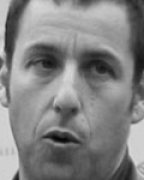
\includegraphics[width=0.09\textwidth]{images/intro/class0_0} &
		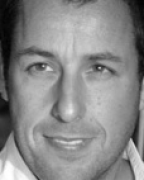
\includegraphics[width=0.09\textwidth]{images/intro/class0_1} & 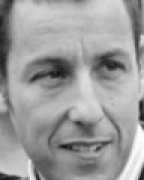
\includegraphics[width=0.09\textwidth]{images/intro/class0_2} & 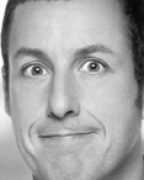
\includegraphics[width=0.09\textwidth]{images/intro/class0_3} & $\cdots$ \\ \hline
		Emma Watson & 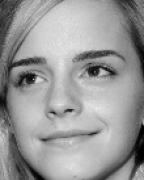
\includegraphics[width=0.09\textwidth]{images/intro/class1_0} &
		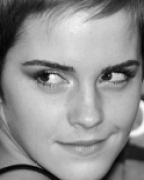
\includegraphics[width=0.09\textwidth]{images/intro/class1_1} & 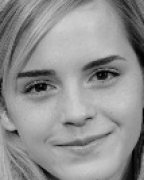
\includegraphics[width=0.09\textwidth]{images/intro/class1_2} & 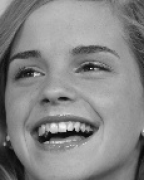
\includegraphics[width=0.09\textwidth]{images/intro/class1_3} & $\cdots$ \\ \hline
		Natalie Portman & 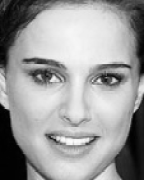
\includegraphics[width=0.09\textwidth]{images/intro/class2_0} & 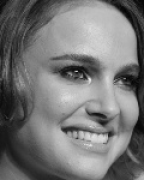
\includegraphics[width=0.09\textwidth]{images/intro/class2_1} & 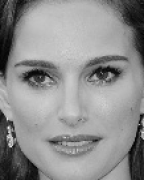
\includegraphics[width=0.09\textwidth]{images/intro/class2_2} & 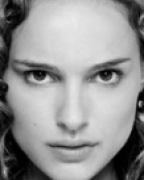
\includegraphics[width=0.09\textwidth]{images/intro/class2_3} & $\cdots$ \\ \hline
		$\qquad\qquad\vdots$ & $\qquad\vdots$ & $\qquad\vdots$ & $\qquad\vdots$ & $\qquad\vdots$ & $\ddots$ \\
	\end{tabular}
\end{frame}

\begin{frame}{Training Set}
	\centering
	\textbf{The code learns how to classify from given \textcolor{blue}{training images}.}\\
	\vspace*{0.5cm}
	\begin{tabular}{l m{1.5cm} m{1.5cm} m{1.5cm} m{1.5cm} c}
		\textbf{Class} & \textbf{Image 1} & \textbf{Image 2} & \textbf{Image 3} & \textbf{Image 4} & $\cdots$ \\ \hline
		male & 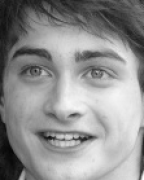
\includegraphics[width=0.09\textwidth]{images/recognition/Daniel_Radcliffe} &
		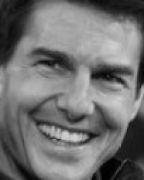
\includegraphics[width=0.09\textwidth]{images/recognition/Tom_Cruise} & 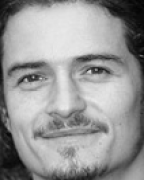
\includegraphics[width=0.09\textwidth]{images/recognition/Orlando_Bloom} & 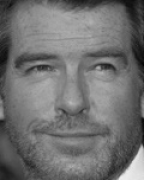
\includegraphics[width=0.09\textwidth]{images/recognition/Pierce_Brosnan} & $\cdots$ \\ \hline
		female & 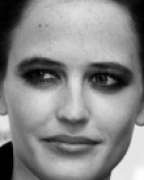
\includegraphics[width=0.09\textwidth]{images/recognition/Eva_Green} &
		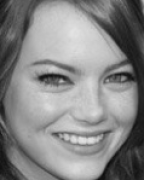
\includegraphics[width=0.09\textwidth]{images/recognition/Emma_Stone} & 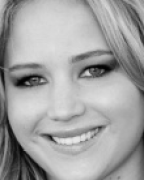
\includegraphics[width=0.09\textwidth]{images/recognition/Jennifer_Lawrence} & 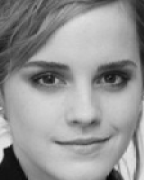
\includegraphics[width=0.09\textwidth]{images/recognition/Emma_Watson} & $\cdots$ \\ \hline
	\end{tabular}
\end{frame}

\begin{frame}[fragile]{Image as Matrix}
\begin{minipage}{0.48\textwidth}
	\begin{columns}[T,onlytextwidth]
		\column{\textwidth}
		\metroset{block=fill}
		\begin{block}{Representation of Grayscale Images}
			Map pixels to values between 0 (black) and 1 (white)
			and represent as $\textcolor{blue}{M}\times\textcolor{green}{N}$
			matrix with entries $p_{ij}\in\left[0,1\right]$.
		\end{block}
	\end{columns}
\end{minipage}\hfill
\begin{minipage}{0.48\textwidth}
	\vspace{0.5cm}
	\begin{tabular}{m{2cm} m{0.5cm} c}
	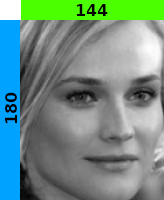
\includegraphics[width=0.3\textwidth]{images/vectormatrix/ImageToVector} &
	$\longleftrightarrow$ &
	$\begin{pmatrix}
		\textcolor{violet}{p_{11}} & \textcolor{orange}{p_{12}} & \cdots & \textcolor{olive}{p_{1N}} \\
		\textcolor{violet}{\vdots} & \textcolor{orange}{\vdots} & \ddots & \textcolor{olive}{\vdots} \\
		\textcolor{violet}{p_{M1}} & \textcolor{orange}{p_{M2}} & \cdots &  \textcolor{olive}{p_{MN}} \\
	\end{pmatrix}$
\end{tabular}\\[0.5cm]
\pause
\end{minipage}
\begin{minipage}{0.48\textwidth}
	\begin{columns}[T,onlytextwidth]
	\column{\textwidth}
	\metroset{block=fill}
		\begin{block}{Example}
			Which image on the right is represented by the following matrix?
			\begin{equation*}
				\begin{pmatrix}
					1 & \frac{1}{4} \\
					\frac{1}{2} & 0 \\
					0 & \frac{3}{4} \\
				\end{pmatrix}
			\end{equation*}
		\end{block}
	\end{columns}
\end{minipage}\hfill
\begin{minipage}{0.48\textwidth}
	\definecolor{onefourth}{rgb}{0.25, 0.25, 0.25}
	\definecolor{onehalf}{rgb}{0.5, 0.5, 0.5}
	\definecolor{threefourth}{rgb}{0.75, 0.75, 0.75}
	\scalebox{0.75}{%
		\begin{tikzpicture}
			\draw[step=1cm,white,very thin] (0,0) grid (2,3);
			\fill[white] (0,0) rectangle (1,1);
			\fill[onefourth] (1,0) rectangle (2,1);
			\fill[onehalf] (0,1) rectangle (1,2);
			\fill[white] (1,1) rectangle (2,2);
			\fill[black] (0,2) rectangle (1,3);
			\fill[threefourth] (1,2) rectangle (2,3);
		\end{tikzpicture}
		\qquad\qquad
		\begin{tikzpicture}
			\draw[step=1cm,white,very thin] (0,0) grid (2,3);
			\fill[black] (0,0) rectangle (1,1);
			\fill[threefourth] (1,0) rectangle (2,1);
			\fill[onehalf] (0,1) rectangle (1,2);
			\fill[black] (1,1) rectangle (2,2);
			\fill[white] (0,2) rectangle (1,3);
			\fill[onefourth] (1,2) rectangle (2,3);
		\end{tikzpicture}
		\qquad\qquad
		\begin{tikzpicture}
			\draw[step=1cm,white,very thin] (0,0) grid (2,3);
			\fill[black] (0,0) rectangle (1,1);
			\fill[onefourth] (1,0) rectangle (2,1);
			\fill[onehalf] (0,1) rectangle (1,2);
			\fill[black] (1,1) rectangle (2,2);
			\fill[white] (0,2) rectangle (1,3);
			\fill[threefourth] (1,2) rectangle (2,3);
		\end{tikzpicture}
	}
\end{minipage}
\end{frame}

\begin{frame}[fragile]{Images as Vectors}
\begin{center}
	%Images of resoplution $\textcolor{blue}{M}\times\textcolor{green}{N}$ can be seen as vectors $\vec{p}\in\left[0,1\right]^{\textcolor{blue}{M}\cdot\textcolor{green}{N}}$.\\[1cm]
	\begin{tabular}{m{2.5cm} m{1cm} c m{1cm} c}
	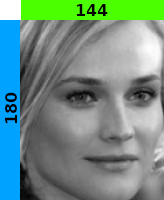
\includegraphics[width=0.15\textwidth]{images/vectormatrix/ImageToVector} &
	$\longleftrightarrow$ &
	$\begin{pmatrix}
		\textcolor{violet}{p_{11}} & \textcolor{orange}{p_{12}} & \cdots & \textcolor{olive}{p_{1N}} \\
		\textcolor{violet}{\vdots} & \textcolor{orange}{\vdots} & \ddots & \textcolor{olive}{\vdots} \\
		\textcolor{violet}{p_{M1}} & \textcolor{orange}{p_{M2}} & \cdots &  \textcolor{olive}{p_{MN}} \\
	\end{pmatrix}$ &
	$\longleftrightarrow$ &
	$\tiny{\begin{pmatrix}
		\textcolor{violet}{p_{11}} \\
		\textcolor{violet}{\vdots} \\
		\textcolor{violet}{p_{M1}} \\
		\textcolor{orange}{p_{12}} \\
		\textcolor{orange}{\vdots} \\
		\textcolor{orange}{p_{M2}} \\
		\vdots \\
		\textcolor{olive}{p_{1N}} \\
		\textcolor{olive}{\vdots} \\
		\textcolor{olive}{p_{MN}} \\
	\end{pmatrix}}$
\end{tabular}
\begin{columns}[T,onlytextwidth]
	\column{\textwidth}
	\metroset{block=fill}
	\begin{block}{Question: What is the following code doing to the image $\vec{p}$?}
		\begin{minipage}{0.45\textwidth}
			\hspace{1cm}
			\lstinputlisting[firstline=19,lastline=23,style=python]{solution/chapter2.py}
		\end{minipage}\hfill
		\pause
		\begin{minipage}{0.2\textwidth}
			\centering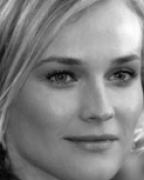
\includegraphics[width=0.6\textwidth]{images/vectormatrix/Diane_Kruger}
		\end{minipage}
		\begin{minipage}{0.2\textwidth}
			\centering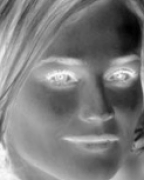
\includegraphics[width=0.6\textwidth]{images/vectormatrix/Diane_Kruger_negative}
		\end{minipage}
	\end{block}
\end{columns}
\end{center}
\end{frame}

\begin{frame}[fragile]{Mean Face and Difference Faces}
	\begin{center}
		We can center the \textcolor{ForestGreen}{training images} around the origin by subtracting the \textcolor{red}{mean face}.
	\end{center}
	\begin{minipage}{0.45\textwidth}
		\begin{tabular}{m{2.0cm} m{0.5cm} c}
			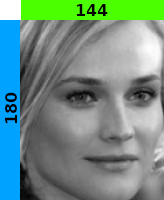
\includegraphics[width=0.3\textwidth]{images/vectormatrix/ImageToVector} &
			$\longrightarrow$ &
			$\begin{pmatrix}
				p_{1} \\
				p_{2} \\
				\vdots \\
				p_{\textcolor{blue}{M}\textcolor{green}{N}} \\
			\end{pmatrix}$ \\
			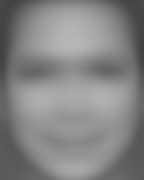
\includegraphics[width=0.3\textwidth]{images/facespace/meanface} &
			$\longrightarrow$ &
			$\begin{pmatrix}
				m_{1} \\
				m_{2} \\
				\vdots \\
				m_{\textcolor{blue}{M}\textcolor{green}{N}} \\
			\end{pmatrix}$
		\end{tabular}
	\end{minipage}
	\begin{minipage}{0.45\textwidth}
		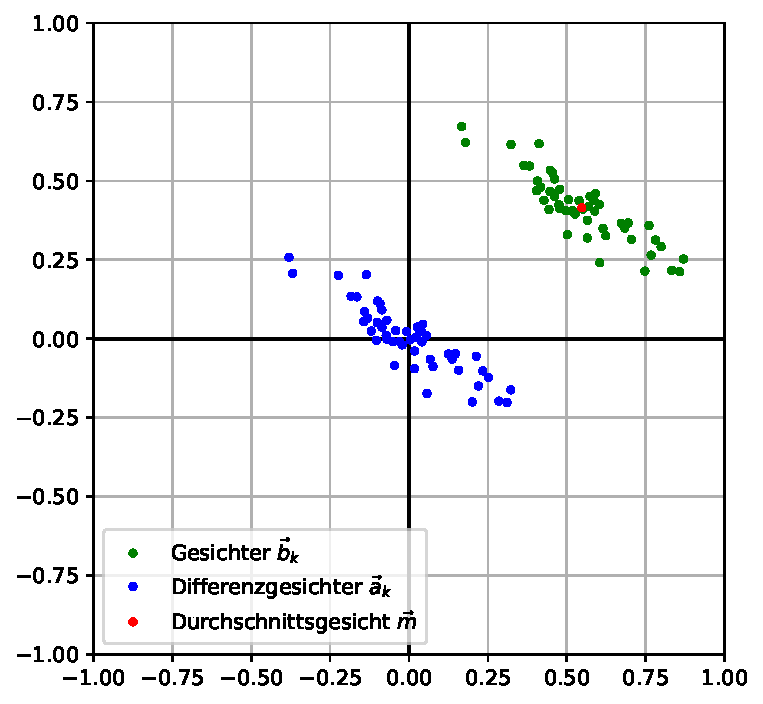
\includegraphics[width=\textwidth]{images/facespace/meandiff}
	\end{minipage}
\end{frame}

\begin{frame}[fragile]{Eigenfaces}
	\begin{center}
		\textcolor{blue}{\textbf{Principal component analysis}} using singular value decomposition yields \textcolor{blue}{\textbf{eigenfaces}}.
	\end{center}
	\begin{minipage}{0.4\textwidth}
		\begin{tabular}{c}
			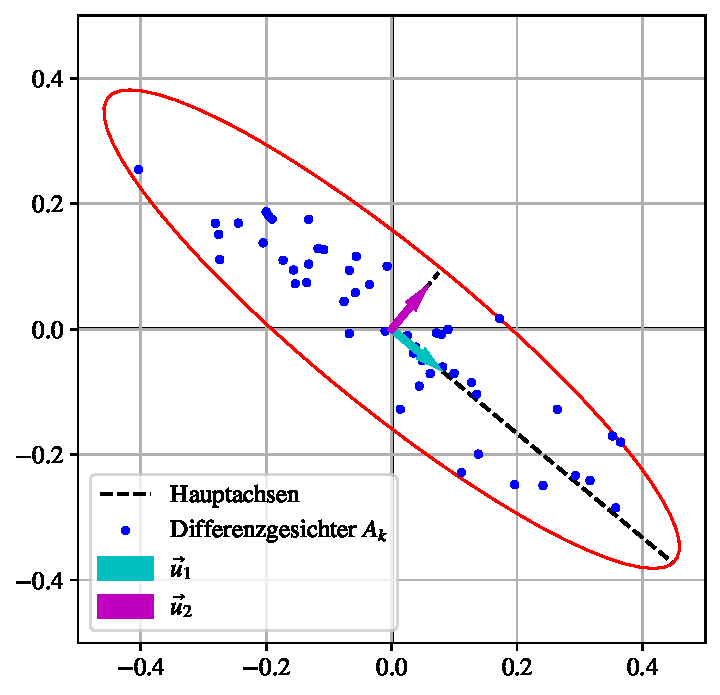
\includegraphics[width=\textwidth]{images/facespace/principal_components}
		\end{tabular}
	\end{minipage}\hfill
	\begin{minipage}{0.45\textwidth}
		\centering
		Eigenfaces as images: $\vec{p}_k=\sigma_k\,\vec{u}_k+\vec{m}$ \\[0.5cm]
		\pause
		\begin{tabular}{cccccccc}
			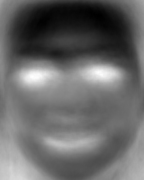
\includegraphics[width=0.18\textwidth]{images/eigenfaces/eigenface00} & 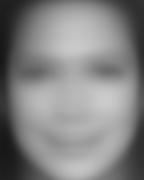
\includegraphics[width=0.18\textwidth]{images/eigenfaces/eigenface01} &
			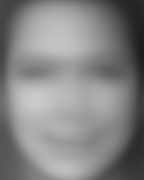
\includegraphics[width=0.18\textwidth]{images/eigenfaces/eigenface02} & 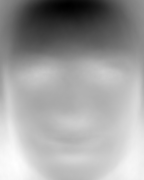
\includegraphics[width=0.18\textwidth]{images/eigenfaces/eigenface03} \\
			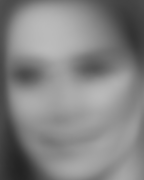
\includegraphics[width=0.18\textwidth]{images/eigenfaces/eigenface04} &
			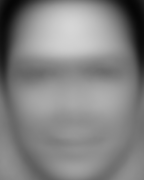
\includegraphics[width=0.18\textwidth]{images/eigenfaces/eigenface05} & 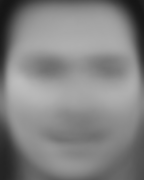
\includegraphics[width=0.18\textwidth]{images/eigenfaces/eigenface06} &
			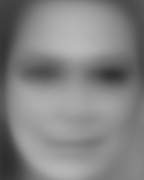
\includegraphics[width=0.18\textwidth]{images/eigenfaces/eigenface07} \\ 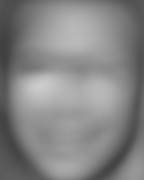
\includegraphics[width=0.18\textwidth]{images/eigenfaces/eigenface08} &
			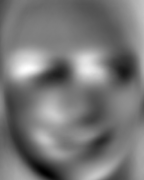
\includegraphics[width=0.18\textwidth]{images/eigenfaces/eigenface09} & 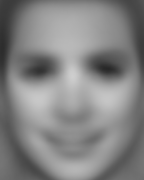
\includegraphics[width=0.18\textwidth]{images/eigenfaces/eigenface10} &
			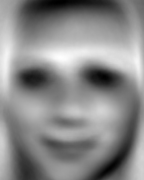
\includegraphics[width=0.18\textwidth]{images/eigenfaces/eigenface11}
		\end{tabular}
	\end{minipage}
\end{frame}

\begin{frame}[fragile]{Transition $\mathbb R^3\longrightarrow\mathbb R^{M\cdot N}$ (projection onto eigenfaces)}
	New face image as supersposition of mean face and eigenfaces:
	$\quad\textcolor{blue}{c_k=\vec{u}_k\cdot\left(\vec{p}-\vec{m}\right)}$\\[0.5cm]
	\begin{tabular}{m{1.3cm} c m{1.3cm} c m{1.3cm} c m{1.3cm} c m{1.3cm} c}
		$\quad\ \ \vec p$ & & $\quad\ \ \vec m$ & & $\quad\ \ \vec u_1$ & & $\quad\ \ \vec u_2$ & & $\quad\ \ \vec u_2$ & \\
		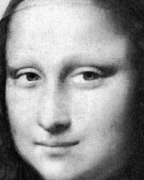
\includegraphics[width=0.1\textwidth]{images/eigenfaces/mona_lisa_eigen_approx} &
		$=$ & 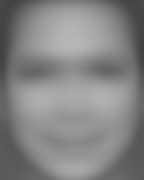
\includegraphics[width=0.1\textwidth]{images/facespace/meanface} & $+\ c_1$ & 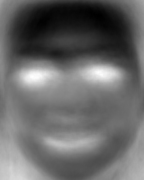
\includegraphics[width=0.1\textwidth]{images/eigenfaces/eigenface00}
		& $+\ c_2$ & 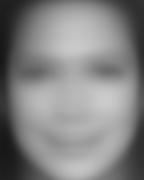
\includegraphics[width=0.1\textwidth]{images/eigenfaces/eigenface01} & $+\ c_3$ & 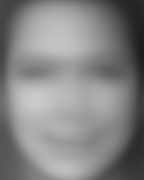
\includegraphics[width=0.1\textwidth]{images/eigenfaces/eigenface02} & $+\ \cdots$
	\end{tabular}\\[0.5cm]
	\pause
	\begin{minipage}{0.45\textwidth}
		\begin{columns}[T,onlytextwidth]
			\column{\textwidth}
			\metroset{block=fill}
			\begin{block}{Use prior knowledge in $\mathbb R^3$}
				\begin{itemize}
					\item linear combination
					\item scalar product
					\item orthogonality
				\end{itemize}
			\end{block}
		\end{columns}
	\end{minipage}\hfill
	\begin{minipage}{0.45\textwidth}
		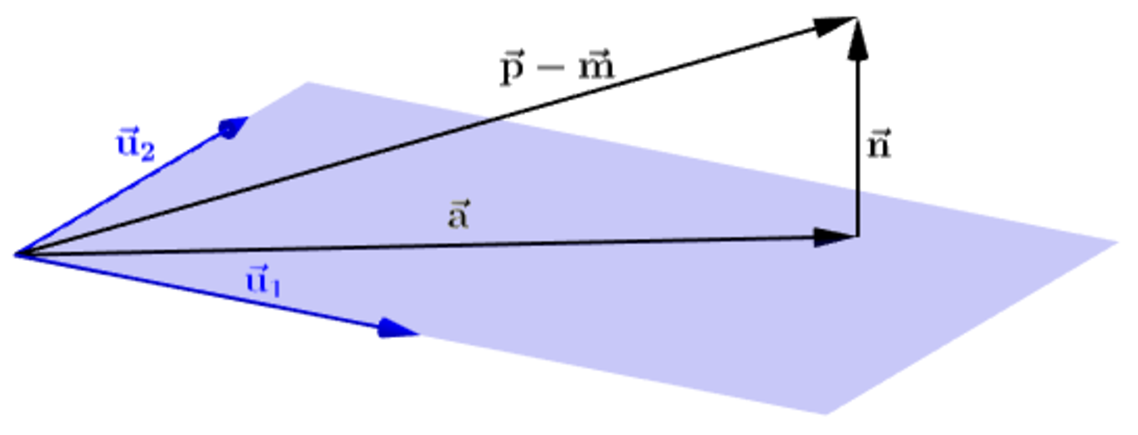
\includegraphics[width=\textwidth]{images/projection2}
	\end{minipage}
\end{frame}

\begin{frame}[fragile]{Eigenfaces vs. Test Images}
	\begin{columns}[T,onlytextwidth]
		\column{\textwidth}
		\metroset{block=fill}
		\begin{minipage}{0.45\textwidth}
			\begin{block}{Observation}
				This can be done with any other (sufficiently large) set of images!
			\end{block}
			\vspace{0.2cm}
			\begin{block}{Question}
				Then what distinguishes the eigenfaces?
			\end{block}
			\vspace{0.2cm}
			Expansion w.r.t. the \textcolor{ForestGreen}{training images}:
		\end{minipage}\hfill
		\begin{minipage}{0.45\textwidth}
			\centering
			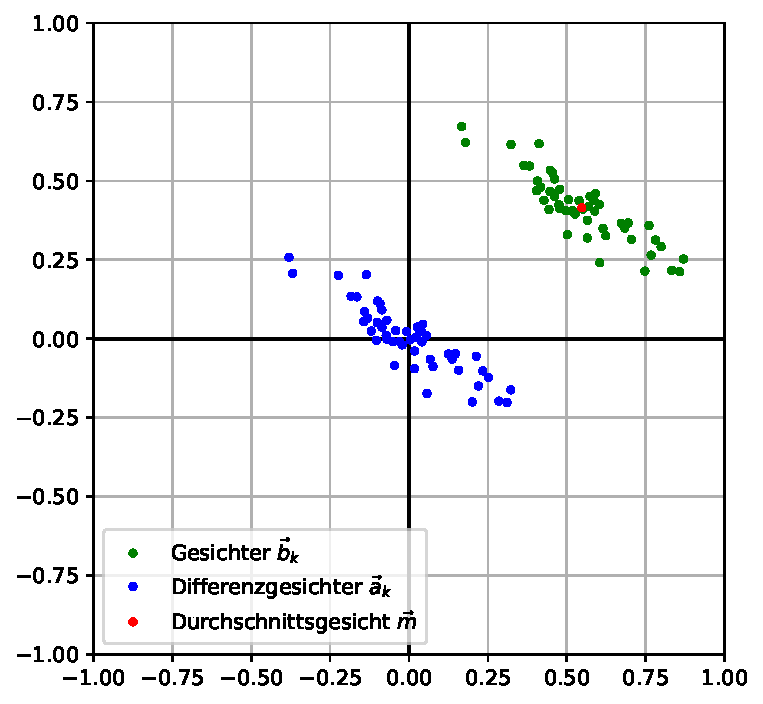
\includegraphics[width=0.7\textwidth]{images/facespace/meandiff}
		\end{minipage}\\
		\vspace{0.5cm}
		\begin{tabular}{m{1.3cm} c m{1.3cm} c m{1.3cm} c m{1.3cm} c m{1.3cm} c}
			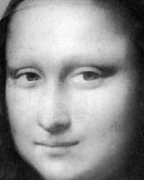
\includegraphics[width=0.1\textwidth]{images/eigenfaces/mona_lisa_naive_approx} &
			$=\ c_1$ & 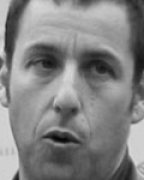
\includegraphics[width=0.1\textwidth]{images/intro/class0_0} & $+\ c_2$ & \includegraphics[width=0.1\textwidth]{images/intro/class1_0}
			& $+\ c_3$ & \includegraphics[width=0.1\textwidth]{images/intro/class2_0} & $+\ c_4$ & \includegraphics[width=0.1\textwidth]{images/intro/class0_3} & $+\ \cdots$
		\end{tabular}
	\end{columns}
\end{frame}

\begin{frame}[fragile]{Image Compression}
	\begin{minipage}{0.65\textwidth}
		\begin{columns}[T,onlytextwidth]
			\column{\textwidth}
			\metroset{block=fill}
			\begin{center}
			Absolute values $\lvert c_k\rvert$ of the \textcolor{blue}{\textbf{coefficients}} of the linear combination w.r.t. the training images and eigenfaces.\\[0.2cm]
			\begin{tabular}{cc}
				\centering
				\includegraphics[width=0.45\textwidth]{images/eigenfaces/naive_coef} &
				\includegraphics[width=0.45\textwidth]{images/eigenfaces/eigen_coef} \\
				\phantom{text}training images & \phantom{text}eigenfaces
			\end{tabular}
			\pause
			\begin{minipage}{0.45\textwidth}
			\begin{block}{Question 1}
				What are the differences?
			\end{block}
			\end{minipage}\hfill
			\pause
			\begin{minipage}{0.45\textwidth}
				\begin{block}{Question 2}
					Are the eigenfaces better?
				\end{block}
			\end{minipage}
			\end{center}
		\end{columns}
	\end{minipage}\hfill
	\pause
	\begin{minipage}{0.3\textwidth}
		\begin{tabular}{m{1.0cm} m{1.0cm} c}
			\includegraphics[width=0.3\textwidth]{images/compression/mona_lisa_20} &
			\includegraphics[width=0.3\textwidth]{images/compression/chair_20} & 20 \pause \\
			\includegraphics[width=0.3\textwidth]{images/compression/mona_lisa_200} &
			\includegraphics[width=0.3\textwidth]{images/compression/chair_200} & 200 \pause \\
			\includegraphics[width=0.3\textwidth]{images/compression/mona_lisa_2000} &
			\includegraphics[width=0.3\textwidth]{images/compression/chair_2000} & 2000 \pause \\ \includegraphics[width=0.3\textwidth]{images/compression/mona_lisa} &
			\includegraphics[width=0.3\textwidth]{images/compression/chair} & original
		\end{tabular}
	\end{minipage}
\end{frame}

\begin{frame}[fragile]{Image Recognition}
	\begin{minipage}{0.65\textwidth}
		\begin{columns}[T,onlytextwidth]
			\column{\textwidth}
			\metroset{block=fill}
			\begin{center}
				\begin{block}{Literature}
					Turk, Pentland, \textit{Face Recognition Using Eigenfaces}, 1991
				\end{block}
				\begin{block}{Task}
					For a given image $\vec{p}$, decide if it shows a face.
				\end{block}
				\begin{block}{Idea}
					If $\vec{p}-\vec{m}$ lies almost in the subspace spanned by the first $K\approx 2000$ eigenfaces, then it is probably a face.
				\end{block}
				\vspace{0.2cm}
				\includegraphics[width=0.6\textwidth]{images/projection2}
			\end{center}
		\end{columns}
	\end{minipage}\hfill
	\begin{minipage}{0.3\textwidth}
		\begin{tabular}{m{1.0cm} m{1.0cm} c}
			\includegraphics[width=0.3\textwidth]{images/compression/mona_lisa_20} &
			\includegraphics[width=0.3\textwidth]{images/compression/chair_20} & 20 \\
			\includegraphics[width=0.3\textwidth]{images/compression/mona_lisa_200} &
			\includegraphics[width=0.3\textwidth]{images/compression/chair_200} & 200 \\
			\includegraphics[width=0.3\textwidth]{images/compression/mona_lisa_2000} &
			\includegraphics[width=0.3\textwidth]{images/compression/chair_2000} & 2000 \\ \includegraphics[width=0.3\textwidth]{images/compression/mona_lisa} &
			\includegraphics[width=0.3\textwidth]{images/compression/chair} & original
		\end{tabular}
	\end{minipage}
\end{frame}

\begin{frame}[fragile]{Gender Recoginition}
	\begin{columns}[T,onlytextwidth]
		\column{\textwidth}
		\metroset{block=fill}
		\begin{minipage}{0.48\textwidth}
			\begin{block}{Task}
				Given an image of a face (any person), determine the gender of the person.
			\end{block}
			\begin{block}{Structure}
				This is a binary classification problem.
			\end{block}
			\pause
			\begin{block}{Approach}
				Use a \textcolor{blue}{separating hyperplane}: Male faces on one side and female faces on the other side.
			\end{block}
		\end{minipage}\hfill
		\begin{minipage}{0.48\textwidth}
			\includegraphics[width=\textwidth]{images/binary_classification/separating_plane_annotated}
		\end{minipage}
	\end{columns}
\end{frame}

\begin{frame}[fragile]{Gender Recoginition}
	\begin{columns}[T,onlytextwidth]
		\column{\textwidth}
		\metroset{block=fill}
		\begin{minipage}{0.48\textwidth}
			\begin{block}{Step 1}
				Compute $\vec{n}\in\mathbb R^{\textcolor{red}{M\cdot N}}$ and $b$, such that
				\begin{equation*}
					\left\{\vec{x}\ \lvert\ \vec{x}\cdot\vec{n}+b=0\right\}
				\end{equation*}
				optimally separates the genders on the training images.
			\end{block}
			\begin{block}{Step 2}
				Given a new image $\vec{p}$, check on which side of the plain it is.
			\end{block}
		\end{minipage}\hfill
		\begin{minipage}{0.48\textwidth}
			\includegraphics[width=\textwidth]{images/binary_classification/separating_plane_annotated}
		\end{minipage}
	\end{columns}
\end{frame}

\begin{frame}[fragile]{Gender Recoginition}
	\begin{columns}[T,onlytextwidth]
		\column{\textwidth}
		\metroset{block=fill}
		\begin{minipage}{0.48\textwidth}
			\begin{block}{Problem}
				Normal $\vec{n}\in\mathbb R^{\textcolor{red}{M\cdot N}}$ has too may parameters to optimize for.
				Recall: $M=180,N=144$
			\end{block}
			\begin{block}{Solution}
				Represent each image by its coefficient vector
				\begin{equation*}
					\vec{c}=\left(c_1,\ldots,c_K\right)^T
				\end{equation*}
				w.r.t. the first $K\approx 2000$ eigenfaces.
			\end{block}
		\end{minipage}\hfill
		\begin{minipage}{0.48\textwidth}
			\includegraphics[width=\textwidth]{images/binary_classification/separating_plane_annotated}
		\end{minipage}
	\end{columns}
\end{frame}

\begin{frame}[fragile]{Didactical Aspects}
	\begin{center}
		\huge{Didactical Aspects:\\ Some Examples}
	\end{center}
\end{frame}

\begin{frame}[fragile]{Transition $\mathbb R^3\longrightarrow\mathbb R^{M\cdot N}$ (Distance Point-Line)}
	\begin{minipage}{0.45\textwidth}
		\begin{columns}[T,onlytextwidth]
			\column{\textwidth}
			\metroset{block=fill}
			\begin{block}{Distance Point-Line in $\mathbb R^2$}
				\begin{itemize}
					\item draw picture
					\item concrete Numbers
				\end{itemize}
			\end{block}
			\begin{block}{Distance Point-Line in $\mathbb R^4$}
				\begin{itemize}
					\item \textcolor{red}{no picture}
					\item concrete numbers
				\end{itemize}
			\end{block}
			\begin{block}{Distance Point-Line in $\mathbb R^{M\cdot N}$}
				\begin{itemize}
					\item \textcolor{red}{picture impossible}
					\item \textcolor{red}{variables instead of numbers}
				\end{itemize}
			\end{block}
		\end{columns}
	\end{minipage}\hfill
	\begin{minipage}{0.45\textwidth}
		\includegraphics[width=\textwidth]{images/facespace/distance_simple}
	\end{minipage}
\end{frame}

\begin{frame}[fragile]{Group work (Setting up the training images)}
	\begin{columns}[T,onlytextwidth]
		\column{\textwidth}
		\metroset{block=fill}
		\begin{block}{Positive Interdependence}
			The more training images, the better the result.
		\end{block}
		\begin{block}{Individual Accountability}
			If somebody provides wrong image files, the whole program won't work.
		\end{block}
		\begin{block}{Promotive Interaction}
			The database is ready only when everyone is done.
			Hence faster students should help the slower students.
		\end{block}
		\begin{block}{Foster Interpersonal Skills}
			Collaboration is only necessary when the results are assembled.
		\end{block}
		\begin{block}{Group Processing}
			Cutting pictures to the right resolution helps to see pictures as $M\times N$ Matrix of pixels.
		\end{block}
	\end{columns}
\end{frame}

\begin{frame}[fragile]{Self-Explanation (Images as Vectors)}
	\begin{minipage}{0.6\textwidth}
		\begin{columns}[T,onlytextwidth]
			\column{\textwidth}
			\metroset{block=fill}
			\begin{block}{Question}
				Name two differences and one similarity of the simplified picture on the right and the real situation (i.e. resolution $M=180$ and $N=144$).
			\end{block}
			\begin{block}{Question}
				Can the difference-faces (\textcolor{blue}{blue}) be rendered to images?
			\end{block}
		\end{columns}
	\end{minipage}\hfill
	\begin{minipage}{0.35\textwidth}
		\includegraphics[width=\textwidth]{images/facespace/meandiff}
	\end{minipage}
\end{frame}

\begin{frame}[fragile]{Further Didactical Aspects}
	\begin{columns}[T,onlytextwidth]
		\column{\textwidth}
		\metroset{block=fill}
		\begin{block}{Scaffolding}
			\begin{itemize}
				\item Computing eigenfaces by SVD is too advanced $\rightarrow$ \textcolor{blue}{eigenfaces as blackbox}.
				\item Loading and saving images has nothing to do with mathematics $\rightarrow$ \textcolor{blue}{code-templates}.
			\end{itemize}
		\end{block}
		\begin{block}{Interleaved practice}
			\begin{itemize}
				\item \textcolor{blue}{blocked}: Develop whole theory first, then write code.
				\item \textcolor{blue}{interleaved}: Alternate between theory and programming.
			\end{itemize}
		\end{block}
		\begin{block}{Holistic mental model confrontation}
			Compare simplified pictures in \textcolor{blue}{3} dimensions with \textcolor{blue}{$N\cdot M$} dimensions.
		\end{block}
	\end{columns}
\end{frame}

\begin{frame}[fragile]{Summary}
	Eigenfaces ...\\
	\vspace{0.5cm} \pause
	\begin{enumerate}[1.] \setlength\itemsep{0.5cm}
		\item ... build on \textcolor{blue}{vector geometry in $\mathbb R^3$}. \pause
		\item ... can \textcolor{blue}{visualize} linear algebra in higher dimensions. \pause
		\item ... can be used as \textcolor{blue}{blackbox}. \pause
		\item ... allow to explore \textcolor{blue}{linear alebra in higher dimensions}.
	\end{enumerate}
\end{frame}
	
\end{document}